% Chapter Template

\chapter{New Model Esitmation and Data Diagnostics} % Main chapter title

\label{Chapter 4} % Change X to a consecutive number; for referencing this chapter elsewhere, use \ref{ChapterX}
\section{Spring Winter Model}
By using the `lm` function from the car package, we find that spring and winter are significant than two other seasons. See:  \refeq{fig:Coefficient Plot}

\begin{figure}[H]
  \centering
  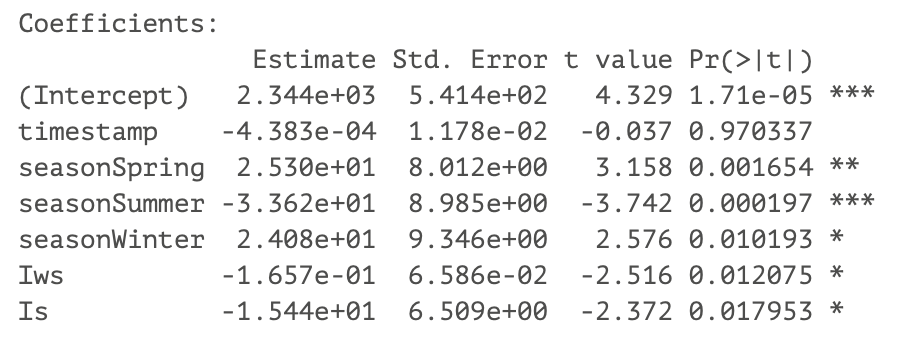
\includegraphics[width = 1.0\textwidth]{Figures/coef_full.png}
  \caption[Figures/coef\_full.png]{Coefficient Plot}
  \label{fig:Coefficient Plot}
\end{figure}

So, we decide to grouping the data into two parts. Spring-Winter data as one set and the Summer-Autumn data as another set. Then we use the lm function to compare these two models and find that the Spring-Winter Model is better than the other one.

\begin{figure}[H]
  \centering
  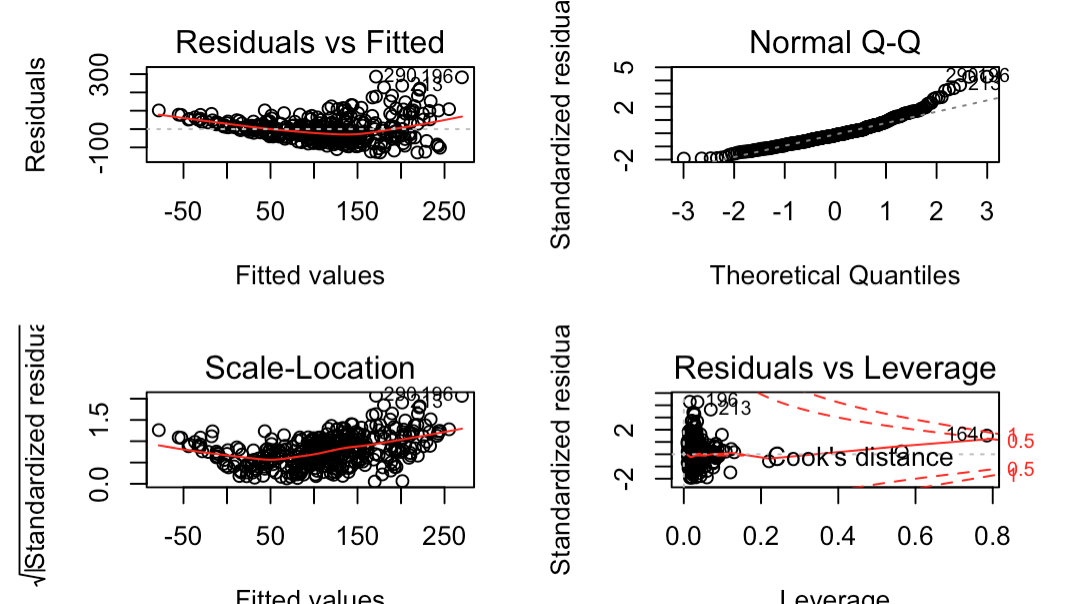
\includegraphics[width = 1.0\textwidth]{Figures/spring_winter.png}
  \caption[Figures/spring\_winter.png]{Spring Winter Model}
  \label{fig:Spring_Winter Model}
\end{figure}


From the plots we can see that there is not linear correlation between these variables. We thus do the ncvTest and draw the spreadlevel plot, the suggested power transformation is 0.381492.\citeq{Kabacoff2015} See: \refeq{fig:NCVTest}

\begin{figure}[H]
  \centering
  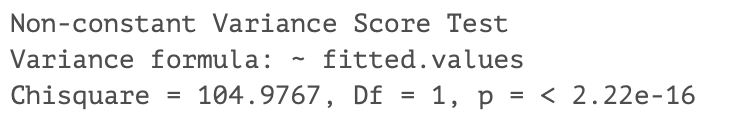
\includegraphics[width = 1.0\textwidth]{Figures/ncv.png}
  \caption[Figures/ncv.png]{NCV Test}
  \label{fig:NCVTest}
\end{figure}

\begin{figure}[H]
  \centering
  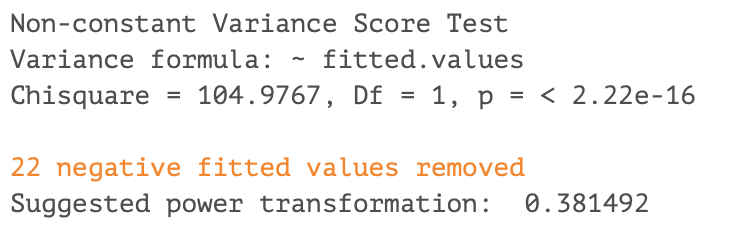
\includegraphics[width = 1.0\textwidth]{Figures/ncv_spread.png}
  \caption[Figures/ncv_spread.png]{NCV Test and Suggested Power Transformation}
  \label{fig:NCV Test and Suggested Power Transformation}
\end{figure}

\begin{figure}[H]
  \centering
  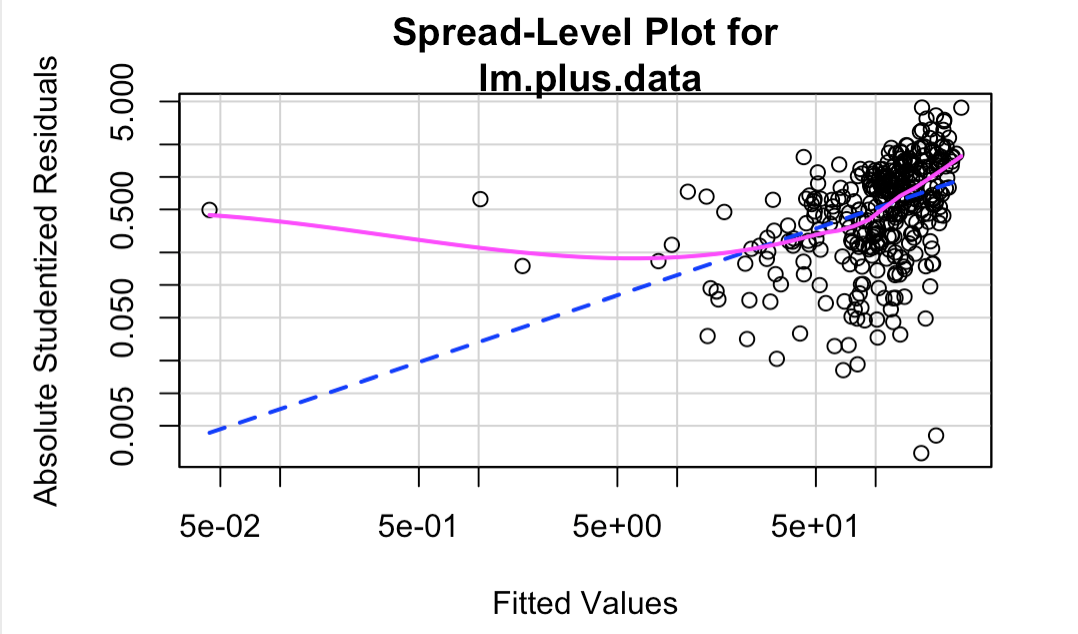
\includegraphics[width = 1.0\textwidth]{Figures/spread.png}
  \caption[Figures/spread.png]{Spreadlevel Plot}
  \label{fig:Spreadlevel Plot}
\end{figure}

. We think it may means closed to $0.5$ or closed to $0$. First, we take square loot to the pm2.5, but the result ignores our consideration. Then we start to consider another possibility, which is closed to $0$, meaning we should take the natural logarithm to the pm2.5. We wonder what will happen if we take the natural logarithm to the pm2.5. We use lm function again to estimate the Spring-Winter Model with natural logarithm and the results shows the linear correlation. Also, the residual plots and the R square are both better than before.

\begin{figure}[H]
  \centering
  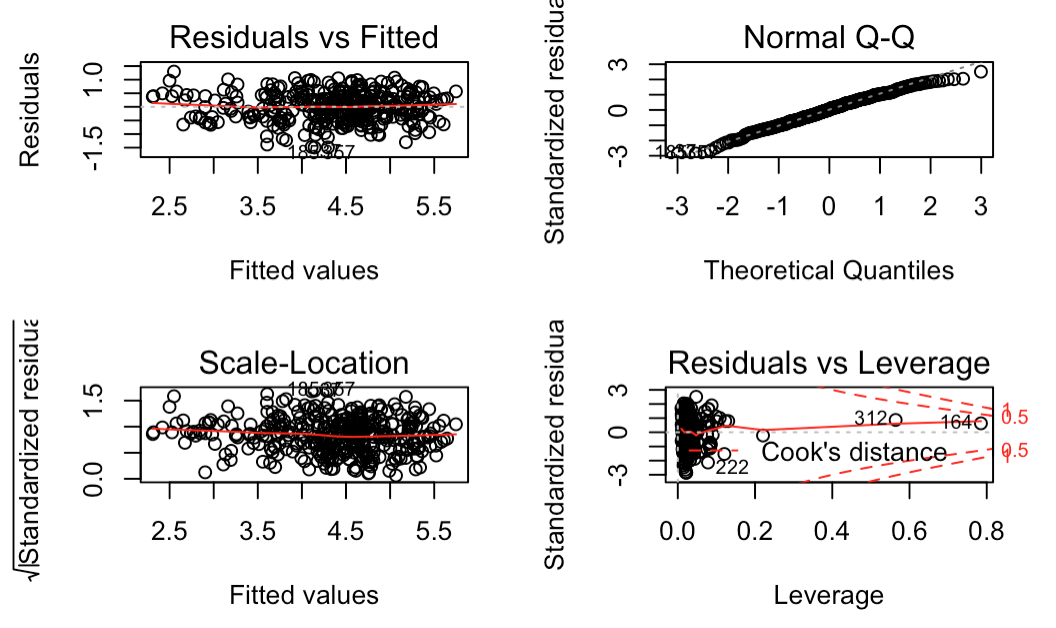
\includegraphics[width = 1.0\textwidth]{Figures/spring_winter_nl.png}
  \caption[Figures/spring\_winter\_nl.png]{Natural Logarithm of Spring Winter Model}
  \label{fig:Natural Logarithm of Spring Winter Model}
\end{figure}

From the full model vif figure, the vif value of the winter is the most significant one in four single seasons. With this discovery, we choose the winter data to form a model with natural logarithm. Also, we form a model for the spring data with natural logarithm, but it is not good as the winter one.

\begin{figure}[H]
  \centering
  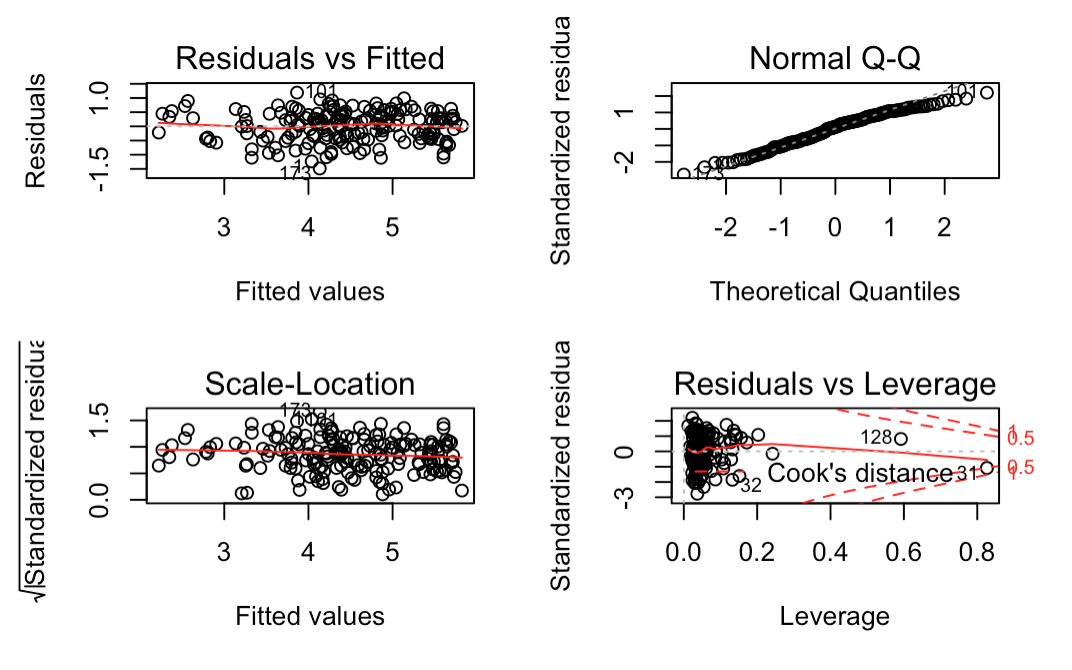
\includegraphics[width = 1.0\textwidth]{Figures/winter_nl.png}
  \caption[Figures/winter\_nl.png]{ Winter Model Natural Logarithm}
  \label{fig: Winter Model Natural Logarithm}
\end{figure}

The Formula of Winter Model with Natural Logarithm is :

\begin{align*}
  log(pm2.5)  = \beta_1 timestamp + \beta_2 Iws + \beta_3 Is + \beta_4 Ir + \beta_5 DEWP +
    \beta_6 TEMP + \beta_7 PRES + \beta_8 cbwd_data \label{eq: Winter Model with Natural Logarithm}
\end{align*}

 The residual plots are better and the R square is higher than what we have found out before.
So we use this model \ref{eq: Winter Model with Natural Logarithm} to do the regression model diagnostics.

\begin{figure}[H]
  \centering
  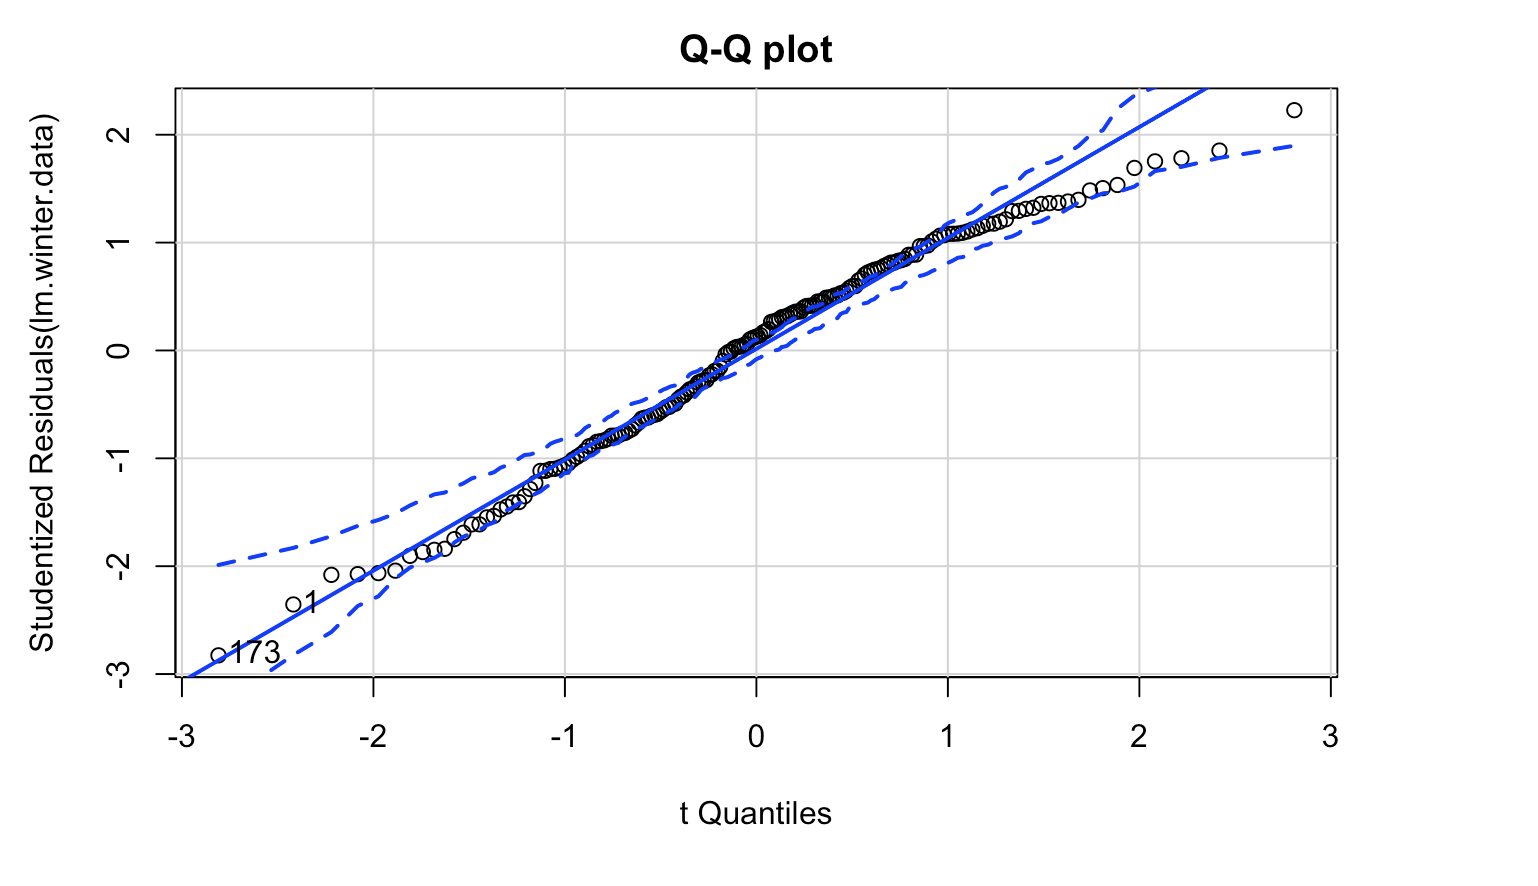
\includegraphics[width = 1.0\textwidth]{Figures/QQ.png}
  \caption[Figures/QQ.png]{Q-Q Plot}
  \label{fig: Q-Q Plot}
\end{figure}

First, we draw the Q-Q plot, the plot shows that all the points are closed to the straight line, and they are all in the confident interval, which means the normality assumption of this Winter Natural Logarithm Model is good.
We also use the residplot function to draw the Studentized Residual Histogram, and add the Normal Curve, Kernel Density Curve and Rug Plot.

\begin{figure}[H]
  \centering
  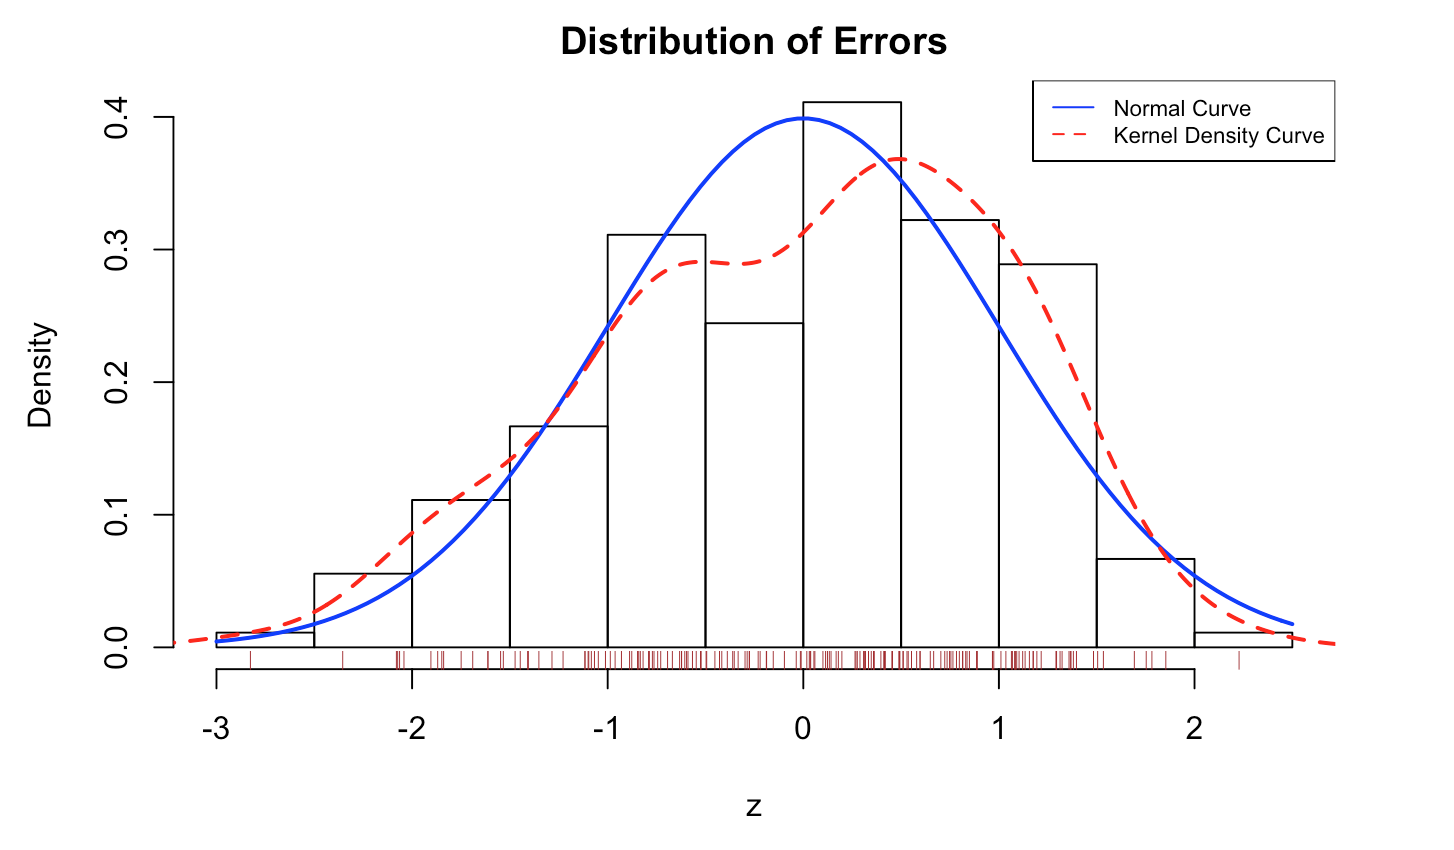
\includegraphics[width = 1.0\textwidth]{Figures/density.png}
  \caption[Figures/density.png]{Studentized Residual Density Plot}
  \label{fig: Studentized Residual Density Plot}
\end{figure}
